\documentclass[final]{beamer}
\mode<presentation>
\usepackage{mathtools}
\usepackage{comment}
\usepackage[english]{babel}
\usepackage[T1]{fontenc}
\usepackage[utf8]{inputenc}
\usepackage{lmodern}
\usepackage{exscale}
\usepackage{amsmath,amsthm, amssymb, latexsym}
\usepackage{caption}

\usepackage{algorithm}
\usepackage{xcolor}
\usepackage{framed}
\usepackage{algpseudocode}
\usepackage{chngcntr}
      % \counterwithout{figure}{chapter}
            \counterwithout{figure}{section}
\usepackage[orientation=portrait,size=a0,scale=1.4]{beamerposter}

\colorlet{shadecolor}{gray!20}

\usetheme[mat, threecolumn]{HYposter}
% Set up the title and author info
\titlestart{Aho-Corasick and Rabin-Karp}
\titleend{in Multiple Pattern String Matching}
\author{Aleksi Hartikainen and Jussi Kokkala}
\leftcorner{}

\begin{document}
\begin{poster}

\newcolumn

\section{Abstract}
Multiple pattern string matching is a common real world problem with applications to virus detection, DNA matching, and plagiarism detection. The task is to find every occurence of each of the given $P$ patterns of combined total length $M$ in a text of length $N$.

Rabin-Karp is a single pattern matching algorithm which can be easily adapted to multiple pattern problem. Aho-Corasick constructs a finite state machine from the pattern set. We implemented both of these algorithms and compared their performance in matching English text patterns.

\section{Rabin-Karp}
      Rabin-Karp uses hashing to find fixed length patterns in a text. The hashing function used is a rolling hash, meaning that the hash of $T[2\;..\;N+1]$ can be calculated from the hash of $T[1..N]$ in constant time. Our implementation uses a hash function which interprets each substring $T[a\;..\;a+N)$ as an $N$ digit number in a base-$B$ numeral system:
\small
\begin{align*}
H_a &= \text{hash}(T[a\;..\;a+N]\;) = \sum_{j=a}^{a+N-1}(T[j] \times B^{a+N-j-1}) \\
H_{a+1} &= \text{rolling\_hash}(H_a, T[a], T[a+N])\\ 
&= H_a \times B -  T[a] \times B^{N}  + T[a+N]
\end{align*}
\normalsize
\vspace{10mm}
\begin{algorithm} [H]
\small
\caption{Single pattern Rabin-Karp}
\label{alg:rk_single}

\begin{algorithmic}[1]
\Require{pattern P of length M, text T of length N}

\State $pattern\_hash \gets \text{hash(pattern)}$
\State $text\_hash \gets \text{hash(T[1\;..\;M])}$
\For {$i \gets M \to N$}
    \If{$ i > M$}
        \State  $text\_hash \gets \text{rolling\_hash(text\_hash,T[i-M],T[i])}$
    \EndIf
    \If{$pattern\_hash = text\_hash $}
        \If{$T[i-M+1\;..\;i] = P$}
            \State $\text{output(i-M+1)}$
        \EndIf
    \EndIf
\EndFor
\end{algorithmic}
\end{algorithm}

If the pattern length is fixed, multiple pattern Rabin-Karp can be modified from algorithm (\ref{alg:rk_single}) by simply storing all pattern hashes in a hash table and checking every text position against each pattern in the hash table at index $text\_hash$.

If the pattern length is not fixed, it is possible to use fixed length Rabin-Karp separately for each pattern length. Another solution is to use the length $L$ of the shortest pattern, and calculate hashes only up to the $L$th character of each pattern. As this increases the number of false alarms, our implementation combines these methods and divides the patterns into several groups of similar lengths.


\section{Aho-Corasick}

Aho-Corasick constructs an automaton (Figure~\ref{fig:ac_machine}), which is then run on the text.
States of this automaton are the nodes of a trie of all patterns.
\newcolumn
\section{}
\vspace{-19mm}
To create transitions for each state and each symbol, the algorithm adds a failure link to each state
(Dotted edges in Figure~\ref{fig:ac_machine}).
Failure links are followed until matching transition is found.
Failure links satisfy following property:

\begin{shaded}
%\begin{mbox}
\textit{
If trie node $v$ corresponds to string $S$, then
$fail(v)$ is the node of the longest suffix of $S$ in the trie.
}
%\end{mbox}
\end{shaded}

%\end{mdframed}

Failure links are created by traversing the trie in breadth first fashion
while using the failure links of previous states to solve each new
link in amortized constant time.
From the root state all failing symbols have self-transitions to make the automaton complete.
%This is shown in algorithm~\ref{alg:ac_fail}

To each accepting state a pattern link (shown green in Figure~\ref{fig:ac_machine})
is added to the longest matching pattern.
From each pattern $s$ there is a link to the longest pattern which
is a suffix of $s$.
Using these links all matching patterns of a node are easily
computed.

Total running time of Aho-Corasick algorithm is $O(N+M)$.
Main disadvantage of Aho-Corasick algorithm is the $O(M)$ space needed to store the automaton.
Our implementation uses $8M+O(P)$ bytes of memory.

%\begin{algorithm} [H]
%\small
%\caption{Running Aho-Corasick automaton}
%\label{alg:ac_run}
%
%\begin{algorithmic}[1]
%\Require{trie, fail, text}
%\State $v \gets \text{root}$
%\For {Each symbol $s$ in text}
%\While {$\text{trie}(v,s)=\bot$}
%    \State $v \gets \text{fail}(v)$ 
%\EndWhile
%\State $v \gets \text{trie}(v,s)$
%\State Output all patterns matching state $v$.
%\EndFor
%\end{algorithmic}
%\end{algorithm}

% \begin{algorithm} [H]
% \small
% \caption{Algorithm for computing failure links}
% \label{alg:ac_fail}
% \begin{algorithmic}[1]
% \Require{Trie of patterns}
% \Ensure{Failure links for all nodes}
% \State $ \text{fail}(\text{root}) \gets \text{fail}$
% \State $Q \gets Queue\{\text{root}\}$
% \While {$Q \neq \emptyset$}
%     \State $v \gets \text{dequeue}(Q) $
%     \For {$s \in \Sigma, \text{trie}(v,s)\neq \bot$}
%         \State $u \gets \text{trie}(v,s)$ 
%         \State $w \gets \text{fail}(v)$ 
%         \While {$\text{trie}(w,s)=\bot$}
%             \State $w \gets \text{fail}(w)$ 
%         \EndWhile
%         \State $ \text{fail}(u) \gets \text{trie}(w,s)$
%         \State $\text{enqueue}(Q,u)$
%     \EndFor
% \EndWhile
% \end{algorithmic}
% \end{algorithm}

%    v = dequeue()
%while (queue is not empty)
%    for each transition (u, s):
%        w = fail[v]
%        while (trie[w][s]==null))
%            w = fail[v]
%        fail[u] = transition[w][s]
%        enqueue(u)
%

\begin{figure}
\centering
 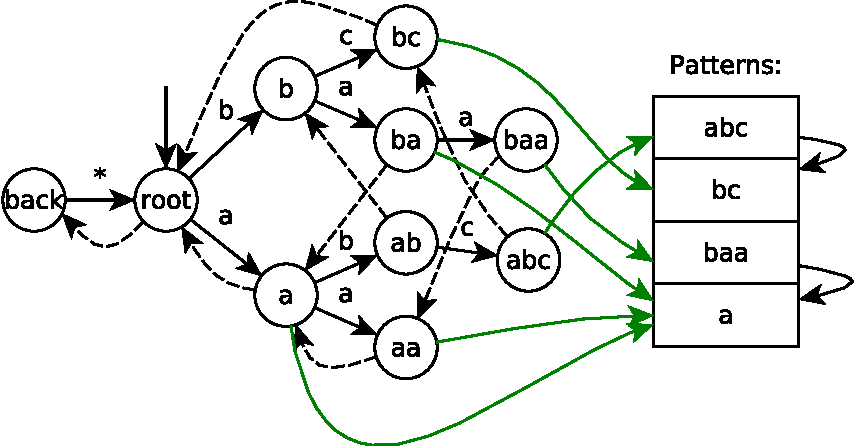
\includegraphics[width=25cm]{aho_corasick.pdf}
\caption{Aho-Corasick automaton with failure links and the associated pattern list}
\label{fig:ac_machine}
\end{figure}

\section{Experiments}
In all our experiments we used the book The Three Musketeers by Alexandre Dumas as the
searched text.
Patterns are selected by randomly sampling a passage from the book.
This ensures that each pattern will produce at least one match.

In figures~\ref{fig:fixed_len} and~\ref{fig:var_len} the searched text is the whole book ($N=1242335$).
%In figure~\ref{fig:fixed_len} Rabin-Karp is faster with longer patterns because the number
%of matches decreases.
%
%When using variable length patterns (Figure~\ref{fig:var_len})
%Aho-Corasick is noticeably faster if total pattern length is small compared to
%pattern length.
%In both cases Aho-Corasick is slower with large pattern sets due to automaton construction.
%If Aho-Corasick automaton is a
% 
In figure \ref{fig:fixed_len} the pattern count is always 30000, but the pattern length is
growing.
In figures \ref{fig:var_len} and \ref{fig:text_len_var} pattern lengths are uniformly randomly selected from the interval $[10,200]$.

\begin{figure}
\centering
 \includegraphics[width=25cm]{fixed_len.pdf}
\caption{Matching time for fixed length patterns with $P=30000$}
\label{fig:fixed_len}
%\caption*{
%}
\end{figure}

\begin{small}
\centering
Rabin-Karp is faster with longer patterns because the number of matches decreases.
Aho-Corasick is slower with longer patterns due to automaton construction.
\end{small}
\newcolumn

\begin{figure}
{\centering
 \includegraphics[width=25cm]{var_len.pdf}
\caption[Matching time for variable length patterns]
{
Matching time for variable length patterns.
\newline
\newline
Rabin-Karp has very low overhead per pattern whereas 
automaton construction dominates 
Aho-Corasick running time.
On the other hand once Aho-Corasick automaton is constructed,
matching is fast even with large pattern sets.
}
\label{fig:var_len}
}
\end{figure}



\begin{figure}
\centering
 \includegraphics[width=25cm]{text_len_fixed.pdf}
\caption{
Search time for fixed length patterns ($M = 200000$ and $P = 10000$)
    \newline
    \newline
This is a good case for Rabin-Karp algorithm, as only one hash length is needed.
}

\label{fig:text_len_fixed}
\end{figure}

\begin{figure}
\centering
\includegraphics[width=25cm]{text_len.pdf}
\caption{
Search time for variable pattern lengths ($M = 100032$ and $P = 951$)
\newline
\newline
Our Rabin-Karp implementation uses 4 different hash lengths with this pattern set.
Aho-Corasick is faster when text length is larger than the total pattern length.
}
\label{fig:text_len_var}
\end{figure}

%\section{Other algorithms}
%There are many algorithms for this problem.
%Most of these algorithms however are limited to patterns of fixed length.

\end{poster}
\end{document}
